\documentclass[12pt, aspectratio=169, xcolor=pdftex]{beamer} 
%%% all LaTeX code must start with a \documentclass statement including its class (e.g. beamer, article)
% aspectratio = either 43 or 169; the latter is for projectors in wide format

%%%%%%%%%%%%%%%%%%%%%%%%%%%%%%%%%% preamble

\usetheme{Darmstadt} 
%%% try other themes, e.g. AnnArbor, Pittsburth, Montpellier, Darmstadt, Berkeley,
%%%                                    CambridgeUS, Dresden, Hannover, Luebeck, Antibes, Madrid... default
\usecolortheme{dolphin}
%%% try other colorthemes, e.g. crane, albatross, seagull, 
%%%             seahorse, dolphin, whale... 
%%%             orchid, rose, lily, ... beetle, ... 

\usepackage{verbatim}
\usepackage{xcolor}
\definecolor{BlueGreen}{cmyk}{0.85,0,0,0.33,0}
\definecolor{ZurichBlue}{rgb}{.255,.41,.884}

\setbeamertemplate{caption}{\insertcaption} %%% to have simple captions

\mode<presentation>

% title and author
\title{\Huge{A brief introduction to beamer}}
\author{\Large{Philip Swallow} \inst{1}  \and \Large{Morris Zapp}\inst{2}}
\institute[Universities of Rummidge and Euphoria] %%% optional
{
 \inst{1} \large{University of Rummidge, UK}
 \inst{2} \large{Euphoria State University, USA}
}
\date{\today}


%\logo{\includegraphics[scale=0.2]{UCL_Logo_DarkBlue.jpg}} %% logo in bottom right corner
\logo{
\includegraphics[scale=0.02]{ctan_lion_600.png}}

%%%%%%%%%%%%%%%%%%%%%%%%%%%%%%%%%%%%%%% end of preamble

%%%%%%%%%%%%%%%%%%%%%%%%%%%%%%%%%%%%%%% begin document

\begin{document}

\maketitle %%% try commenting this line out


\begin{frame}{Overview}
\tableofcontents
\end{frame}


\section{Lists}
\begin{frame}{Itemize and enumerate}
Lists and numberd lists can be nested; use the itemize and
enumerate environments

\begin{itemize}
\item{First level}
\begin{enumerate}[I]
\item Point A
\item Point B
\begin{enumerate}[i]
\item part 1
\item part 2
\end{enumerate}
\item Point C
\item Point D
\end{enumerate}
\item{Second level doesn't have any other lists}
\end{itemize}
\end{frame}

\begin{frame}{overlays using \lq\ - \ \rq}
\begin{itemize} %%% the ``-'' means ``and following slides''
    \item<1-> {This is on the first and all following slides}
    \item<2-3> {This is on the second, and third slides}
    \item<3> {This is on the third slide only}
    \item<1,4> {This is on the first and  fourth slide only}
    \item<1-2, 5-> {This is on the first and second, and fifth and following slides}
    \item{All slides}
\end{itemize}
\end{frame}


\begin{frame}{overlays using \lq\ +- \ \rq}
  \begin{itemize} %%% avoids counting:  using <+-> all items appear sequentially
    \item<+-> This is on the first and all following slides
    \item<+-> This is on the second and all following slides
    \item<+-> This is on the third and all following slides
 \end{itemize}
\end{frame}

\section{Figures}
\begin{frame}{Add a figure}
\centering{
   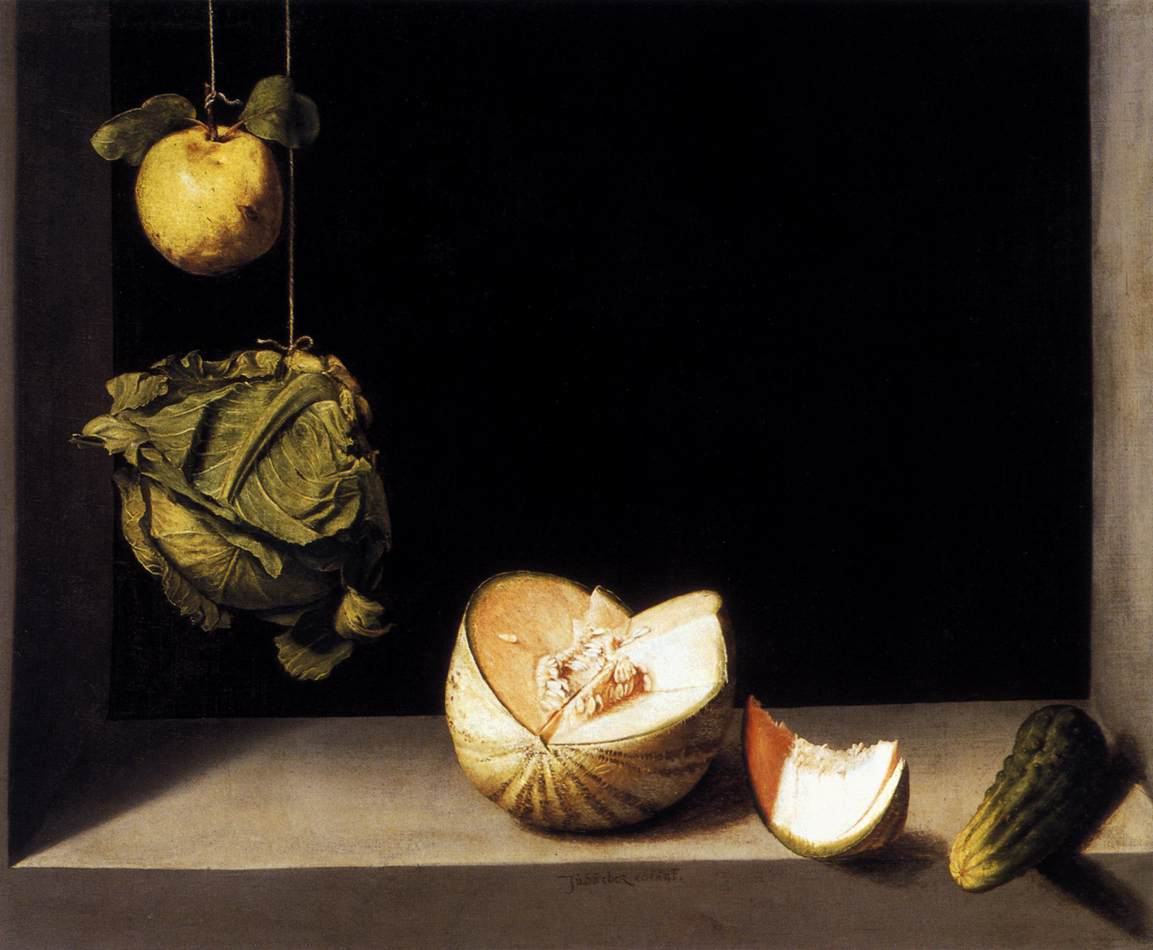
\includegraphics[scale=0.6]{Still_Life_Hyperbola.jpg}\\ %%% change the scale; \\ is carriage return
   \emph{Still Life with Quince, Cabbage, Melon and Cucumber\\ c1602 (290 cm x 239 cm)
    by Juan S\'anchez Cot\'an.  San Diego Museum of Art} %%% see the effect of \emph
 } %%% close centering
\end{frame}

\section{Equations}
\begin{frame}{Add equations}
\begin{itemize}
\item{Equations in \TeX \ and \LaTeX\  are written between \$ signs}
\item{For instance, 
$A\,(r) = \pi\,r^2$ is the area of a circle with radius $r$}
\item{It's easy to write aligned arrays of equations:}
\begin{eqnarray*} % the * suppresses automatic numbering
Y \sim  \mathcal{N}\left(\mu,\,\sigma^{2}\right) & \Rightarrow & 
f_Y\,\left(y; \mu,\sigma^{2}\right) = 
\frac{1}{\sigma \sqrt {2\pi }}
e^{ \left(x - \mu \right)^2\,/\,2\sigma^2}, \\
 & & \rm{and}\  \rm{E} (Y) = \mu, \rm{var}(Y) = \sigma^2 \\
\end{eqnarray*}

\end{itemize}
\end{frame}

\section{Columns and colours}
\begin{frame}{Columns and colour}
\centering{\huge{\color{BlueGreen}{Two compositions with conic sections}}}
\begin{columns}
  \begin{column}[T]{0.5\textwidth}
  \centering{
       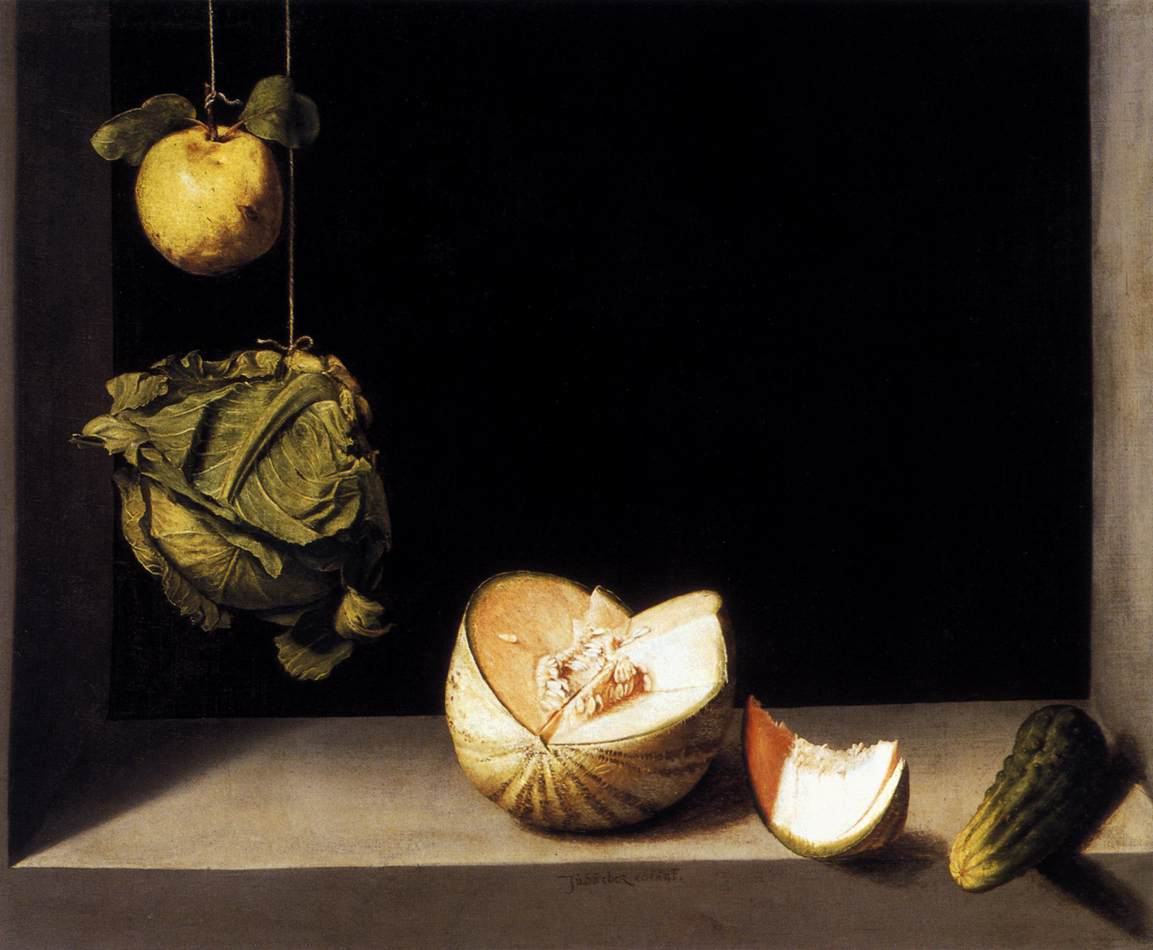
\includegraphics[scale=0.35]{Still_Life_Hyperbola.jpg}
}\\ %%% end of \centering
       \tiny{\emph{Still Life with Quince, Cabbage, Melon and Cucumber\\ c1602 ($290 \times 239$ cm)
    by Juan S\'anchez Cot\'an.  San Diego Museum of Art}} %%% see the effect of \tiny, \small and \emph

  \end{column}
  \begin{column}[T]{0.5\textwidth}
       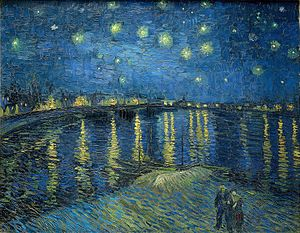
\includegraphics[scale=0.35]{Starry_Night_Over_the_Rhone.jpg}\\
       \tiny{\emph{Starry Night over the Rh\^one\\
       c1888 ($72.5 cm \times 92$ cm) by Vincent van Gogh. Mus\'ee d\rq Orsay, Paris}}
   \end{column}
 \end{columns}
\end{frame}

\begin{frame}[fragile]{More on colours}
%%% option fragile allows using the \verbatim environment
%%% sometimes if something doesn't work, use this  option in the
%%% frame

To change the \textcolor{red}{colour of text} use the command

\begin{verbatim}
\textcolor{colour}{text}
\end{verbatim}

To highlight \colorbox{red}{text} use the command
\begin{verbatim}
\colorbox{highlight colour}{text}
\end{verbatim}


To highlight 
\colorbox{red}{\textcolor{yellow}{text of a different colour} }
use the command
%%% note the effect of leaving an empty line after "To highlight"

\begin{verbatim}\colorbox{red}{\textcolor{yellow}{text}}
\end{verbatim}


To create a \fcolorbox{red}{yellow}{text box with a border}
use the command

\begin{verbatim}\fcolorbox{red}{yellow}{text}
\end{verbatim} %%% \end{verbatim} must be in a separate line

\end{frame}

\section{Tables}
\begin{frame}{Tabular environments}
\begin{itemize}
\item{The tabular environment defines tables}
\item{The table environment defines properties of the table, e.g.
caption}
\end{itemize}


\begin{table}[h] %%% try changing [h] (here) for [t] (top of the page)
\begin{tabular}{c | r | r | r| r} %% defines five columns
%%% first one is center-justified, the rest are right-justified
%%% columns are separated by & and must finish with \\
% \multicolumn{1}{c}{\ } &  \multicolumn{4}{c}{Greek letters}\\ %%% try this instead of the line below
 &  \multicolumn{4}{c}{Greek letters}\\
Name & $\alpha$ & $\beta$ & $\gamma$ & $\delta$ \\
\hline \hline
$N_1$ & 13 & 24 & 18 & 55 \\
$N_2$ & 8 & 22 & 23 & 53 \\
$N_3$ & 14 & 28 & NA & NA \\
$N_4$ & 9 & 21 & 24 & 54 \\
\hline \hline
\end{tabular}
\caption{A random table}
\end{table}



\end{frame}

\end{document}

